\documentclass[conference]{IEEEtran}
\IEEEoverridecommandlockouts
% The preceding line is only needed to identify funding in the first footnote. If that is unneeded, please comment it out.
\usepackage{cite}
\usepackage{amsmath,amssymb,amsfonts}
\usepackage{algorithmic}
\usepackage{graphicx}
\graphicspath{{./}}
\usepackage{textcomp}
\usepackage{xcolor}
\usepackage{url}
\def\BibTeX{{\rm B\kern-.05em{\sc i\kern-.025em b}\kern-.08em
    T\kern-.1667em\lower.7ex\hbox{E}\kern-.125emX}}
\begin{document}

\title{Video Games Sales Analysis\\
}

\author{\IEEEauthorblockN{Dev Rajeshbhai Hathi}
    \IEEEauthorblockA{\textit{Department Of Computer Science And Engineering} \\
        \textit{PES University}\\
        Bangalore, India \\
        devrhathi@gmail.com}
    \and
    \IEEEauthorblockN{Harsha R Patil}
    \IEEEauthorblockA{\textit{Department Of Computer Science And Engineering} \\
        \textit{PES University}\\
        Bangalore, India \\
        harshapatil.karate2001@gmail.com}
}


\maketitle

\begin{abstract}
    This project summerizes region specific impact of genre on the video games sales and the impact of exclusivity on gaming platform sales.  In the first stage of the project report, we aim to exhibit problem statement synopsis, explain the databases and relations among them by an Exploratory Data Analysis.\\
    In the latter stage, we further explore the dataset and get a thorough understanding, which will help us create a better model for prediction of the sales.
\end{abstract}

\begin{IEEEkeywords}
    video games, sales, consoles, exclusivity, genre, region, sales prediction
\end{IEEEkeywords}

\section{Introduction}
The video game industry has grown from niches to mainstream in past few years, having a significant contribution on the global sales market. The number of video games being developed, is showing an exponential growth. The market had a 20\% year-to-year growth from 2019, reaching over \$179 billion in global revenue in both hardware and software for 2020\cite{b1}.  Data analysis for video game business can become large scaled, personalized and real-time. The
statistical processing and Exploratory Data Analysis (EDA) are mainly performed on the data of game platforms, years of distribution and genres.\\
There are number of factors that can potentially affect the sales. Some of them would be:
\begin{itemize}
    \item Popularity of respective consoles
    \item Region
    \item Marketing budget
    \item Genre
    \item Number of positive reviews
    \item Required technical specifications
    \item Popularity of respective platform
\end{itemize}
In our project, we will be estimating the sales of video games and the sales of consoles (platforms). The analysis of video games sales, we will consider Region and Genre and for the sales of respective platforms, we will conduct a special analysis for which, exclusive games will be a primary factor for the sales.\\ The reason for considering exclusive games is because a very popular game being exclusive to a certain platform can potentially drive a lot of console sales since the primary use of a console is to play video games.\\
In the latter stage, we will infere the resultant statistics from the predictions made and make various conclusions such as prioritizing genres or regions for high sales. Which could help optimize marketing strategy and can potentially decrease marketing budget.\\
This project demonstrates that it is a worthwhile direction to analyse the sales for the investigation of business strategies for the publishers in conjunction with the market.

\section{Literature Review}
\textit{What is the effect of Youtube Reviews on Video Games Sales?}\\
This research paper endeavors to identify if YouTube video reviews are more effective than written reviews by critics or users since they are more vivid and informative. The effects of YouTube review videos created by a user and a firm will be investigated. Their effect will be compared to textual online reviews by critics and consumers. Since videos are vivid and create better visuals about a game experience, YouTube review videos are very likely to have a high impact on video game sales. This is why they should be investigated. It is a timely topic for the video gaming industry to understand the importance of YouTube video reviews for the success of a newly released game. Findings from this research can help game developers and video games companies to plan their marketing strategies, spending efficiently and target the right channels for optimal sales performance. Compared to professional critics and ordinary consumers, YouTube influencers provide more reliable and trustworthy information.\\
The following ordinary regression model was fitted:\\
\begin{figure}[h]
    \centering
    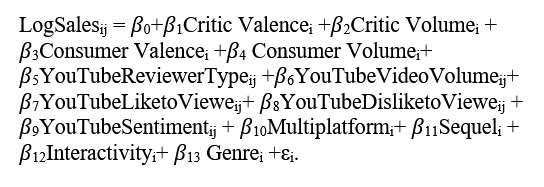
\includegraphics[width=0.5\textwidth]{L1F1.jpg}
    \caption{Formulae 1}
\end{figure}

Where i indicates a video game title and j represents the YouTube video index. Standardized values will be used in regression due to different units of measurement.\\
Some of the Hypothesis Argumentation considered in this paper are:\\
\begin{itemize}
    \item H1: YouTube video posted by an influencer has higher game sales than YouTube video posted by a firm.
    \item H2: There is a positive relationship between consumer engagement behaviours on YouTube and game sales.
    \item H3: The effect of YouTube videos on game sales is higher than the effects of ordinary and critic reviews.
    \item
\end{itemize}
Additionally, being a multiplatform video game, belonging to the action genre, and being a multiplayer game increased video games sales. Thus, H1 was not confirmed and H2 was confirmed for total views and like/dislike to view ratio, but not for YouTube sentiment.\\
H3 was not confirmed because the impact of valence of consumer reviews was significantly higher than any of consumers YouTube engagement indicators.\\
As a social media engagement indicator, the number of YouTube views and likes/dislikes is useful for increasing sales.\\
In these results, volume, and positive assessments of a new game by consumers, volume of critic reviews, high number of YouTube review videos, and engaging YouTube review videos can help companies to increase their game sales. Besides, the effectiveness of content posted by users compared to content posted by companies did not differ.\\
This research signified the evidence to support the role of YouTube reviews as an effective communication channel for marketing managers of gaming companies and game developers. Increase YouTube reviews that have high consumer engagement, and select YouTube reviewers with high engagement for further publicity and promotions. Reviews by consumers and critics should not be undervalued because they have the highest positive effects.\\
\hfill \break
\textit{What is the Impact of Platform on the global sales of Video Game titles?}\\
The purpose of this research paper is to analyse the video games industry with a focus on the comparison of the global sales of different gaming platforms. The approach here is to compare global video game sales by their platform for the duration period 2006 through 2011.\\
Based on the annual sales, the data consists of the top 100 selling video game platforms Nintendo DS, Nintendo GameCube, PC, Sony PlayStation 2, Sony PlayStation 3, Sony PlayStation Portable (PSP), Nintendo Wii, and Microsoft Xbox 360.\\
The paper starts with the Introduction to various terms, then goes through a brief history of video games and consoles. The history gives us a brief introduction to generations of consoles starting from First Generation Consoles all the way to Seventh Generation Consoles. Then after a quick comparision among all Seventh Generation consoles, handheld consoles, the method of statistics used in this paper is described.\\
The statistical methodology incorporates a nonparametric approach for the comparision of video game sales across gaming platforms. The non-linearity of the data moving from sixth to sevent generation console sales, makes it difficult for us to use a traditional regression model. So, the test that is instead used, is Kruskal-Wallis test since it offers the most powerful test statistic in a completely randomized design without assuming a normal distribution. It is sensitive to differences among means in the k populations and is useful when the alternative hypothesis is that the k populations do not have identical means. The null hypothesis is that the k video game sales on the different platforms come from an identical distribution function.\\
\begin{figure}[h]
    \centering
    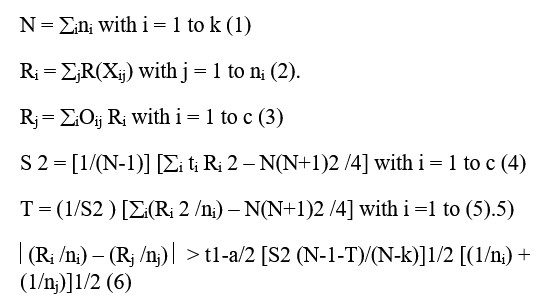
\includegraphics[width=0.5\textwidth]{L2F1.jpg}
    \caption{Formulae 2}
\end{figure}
In the equations here, R is the variable rank and N is the total number of observations. The first three equations find average ranks. Fourth equation calculates the sample variance while the fifth equation represents the test statistic T. If the decision is to reject the null hypothesis, sixth equation determines multiple comparisons of video game sales across various platforms.\\
Despite the observation that the Nintendo Wii is the leader in video game sales, being technical specifications wise superior, the Xbox 360 and Sony PlayStation 3 is not ignored by ``gamers''.\\
While a gaming personal computer (PC) platform will offer far better graphical capabilities than ANY of these consoles, hardware prices for these machines are usually much higher than the price of a console. Despite being a costly machine, the statistics shows that the market continues to value the PC as a gaming platform\\
An interesting focus point for the future will be the battle for portable mobile hand-held market. The mobile devices are making significant inroads into the hand-held market.\\
The results show clear differences in sales by platform along with the brand lines. Nintendo is clearly the gaming leader in this paper with Nintendo Wii as the dominant console and DS being the leading hand-held platforms. Although, being a late arrival, Sony has its own advancements like HD Picture quality and better frame rates (FPS) for more visually appealing experience, Motion Sensing Controllers allowing gamers to experience more immersion etc. portability considerations for their hand-held consoles. \\
Another avenue for future research is to explore the potential for mergers and acquisitions in the video game industry. The timing is ripe for a new console company to enter in the market who understands both hardware and online delivery.\\
\hfill \break
\textit{What were the Strengths, Weakness, Opportunities and Threats on Sony PlayStation during the COVID-19?}\\
By using the SWOT analysis model, the paper studies the sales and development of PlayStation in the context of the pandemic and tries to determine whether the pandemic has any positive implications for customers' living situations. SWOT stands for Strengths, Weakness, Opportunities and Threat.\\
1. Strengths:\\
First of all, PlayStation has a huge number of exclusive games which means players can only play those games in the PlayStation platform.\\
Secondly, in addition to the exclusive games on PlayStation, customers can get a totally different experience when playing those games that can be played on other platforms with PlayStation.\\
Lastly, PlayStation's customer service is excellent, and the system is extremely easy to use. PlayStation's device has a relative longer life because of its backward compatibility. Sony’s PlayStation is the second-best alternative choice for a gaming PC. Customers will always be attracted to cost-effectiveness. \\
2. Weakness:\\
We know that price of the console is lower than PC's, but the price of games should be considered. Because, games on the PlayStation platform have higher prices. PlayStation does provide keyboard and mouse to rival PC gaming, but it is not up to the mark and the experience is not as smooth as controller.\\
3. Opportunities:\\
Sony can catch the market changes of the pandemic and has made some positive improvement on the PlayStation. As is offers Play at Home activity that give some free games to gamers and encourage customers to spend more time at home to protect themselves. The higher price of NVidia graphic cards also encourages people to choose console instead of PC. Apart from gaming, PlayStation can be used as movie and show watching platforms as well.\\
4. Threats:\\
Other platforms and their sales are threats to PlayStation. Only limited number of customers can get their own console because of the sales number. And it gives rise to the high price in the second market platform like Stockx and eBay. Sometimes, the fraud may also happen.\\
Few Recommendations\\
The console for sale is now less but the demand of the customer is in large amount. Increasing the production rate would be very beneficial. Secondly, Sony should cut down the price of the game on its platform. The games on PlayStation platform now are higher than games on almost all other platforms.Third, the exclusive games now are too limited. Compared with hundreds of exclusive games on Switch and PC.\\
In short, against the backdrop of the pandemic, Sony's PlayStation had good development and sales prospects as people stayed at home and needed something to relax with. The company also took steps to attract more customers with its Play At Home promotion, where customers can play games for free.If Sony can make some changes and follow the recommendations, more customers will choose Sony and the company's revenue will increase to a great extent. Maybe in the future, Sony should overcome the threats listed in the model so that the sales of PlayStation console will be more successful.

\section{Exploratory Data Analysis}
Before coming up with the potential sales prediction idea, the data had to be explored and analysed. The datasets used for this analysis were scraped from \cite{b2}. The datasets are:
\begin{itemize}
    \item vgsales - Video Games Sales \cite{b3}
    \item console - Console Sales \cite{b4}
\end{itemize}
Here, in the Console Sales, the ConsoleID is used as a foreign key for joining the video games sales dataset to this dataset and the number of sales are acquired from Wikipedia\cite{b5}. We had to take a closer look at what the data can tell us beyond the formal modeling and thereby contrasting traditional hypothesis testing. We started by pre-processing the data and made it completely usable. Then, we began answering many questions using the data such as:
\begin{itemize}
    \item What are the most sold games globally?
    \item Which was the best performing regions?
    \item What were the best selling consoles?
    \item What are the games that released way back but still being a major player in terms of sales?
    \item What are the top genres that are dominating the global sales?
\end{itemize}
The statistical answers and visualizations gave us very detailed insights in the data.\\
Quite unsurprisingly, the title Wii Sports was the best selling one. Following to that, we have Grand Theft Auto V, Super Mario Bros, Tetris etc as seen in the figure below\\
\begin{figure}[h]
    \centering
    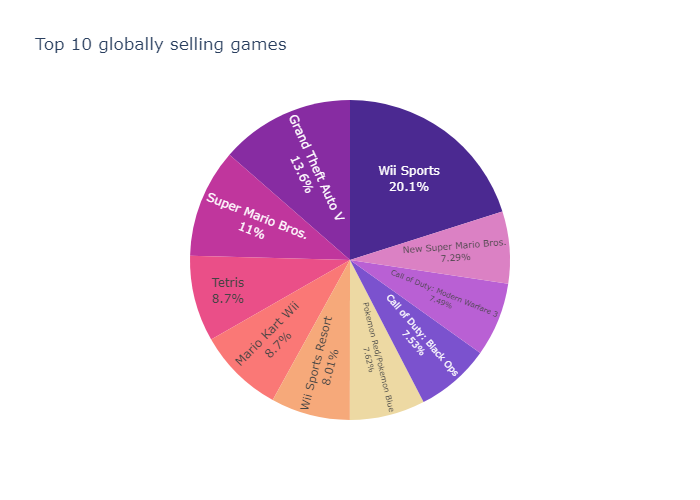
\includegraphics[width=0.5\textwidth]{top10games.png}
    \caption{Top 10 Highest Selling Video Games}
\end{figure}
North America is the biggest contributor in terms of average sales, having \$264,667.43M US Dollar Sales, Which is almost double the times of sales of the second biggest contributor, Europe (\$146,652.01M US Dollars). Then, the top performing genres are Action, contributing a strong \$1751 million USD sales. Sports being the second and followed by Shooter, Role-Playing and Platform genres. Although, these genres sales statistic can be quite baffling, as few titles having a big contribution among all games are not among these top genres. Then, we began analysing the top 1\% of games that were released before 2000. Here, Super Mario Bros, Tetris, and Pokemon Red/Pokemon Blue are among the top 7 selling games of all time! Having \$45.31M, \$35.84M and \$31.37M US Dollar Sales respectively, they are still keeping their toes dipped in the competition with the newly launched video games. While action being the dominating genre in terms of sales, contribution of all genres are almost equal when it comes to top-selling video games globally. \\
There is some interesting diversity when it comes to top consoles in the regions. North America has Xbox 360, Europe has PlayStation 3 and Japan has DS as their top-selling consoles. These top consoles influence region wise most sold game titles. Having the highest cumulative sales, PlayStation 2 is the most sold console globally. Overall sales of every platform in each region can be seen in the figure below.\\
\begin{figure}[h]
    \centering
    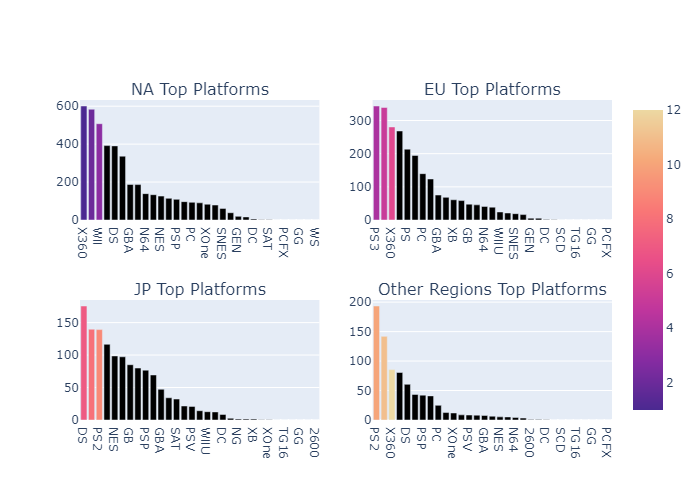
\includegraphics[width=0.5\textwidth]{regionplatform.png}
    \caption{Region Wise Top Selling Platforms}
\end{figure}

While Wii Sports is the top selling game among all regions, Japan is an exception. This might be due to the title being exclusive to Wii Consoles and Japan having very less Wii console sales when compared with other regions. Although Japan's contribution in the sales of the title Pokemon Red/Pokemon Blue is quite big. This title is not even among the top 5 games in other regions, yet it is making it to top 7 video games. Again, exclusivity comes into picture for this, since this title is exclusive to DS consoles for which, Japan is the biggest consumer.\\
Then we proceeded to analyse the top genres dominating the sales. From the figure below, we can see that action is a clear winner, followed by Sports, Shooter and then role-playing.\\
\begin{figure}[h]
    \centering
    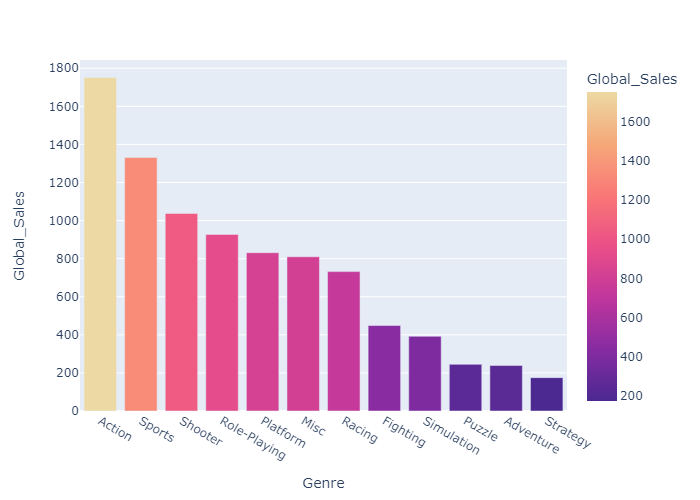
\includegraphics[width=0.5\textwidth]{totalgenre.png}
    \caption{Global Top Selling Genres}
\end{figure}\\
However, a better analysis for the top genres would be considering them region wise. Since there is a big diversity among regions when it comes to genres. Here are the top genres based on two of the most popular new generation gaming consoles.
\begin{figure}[h]
    \centering
    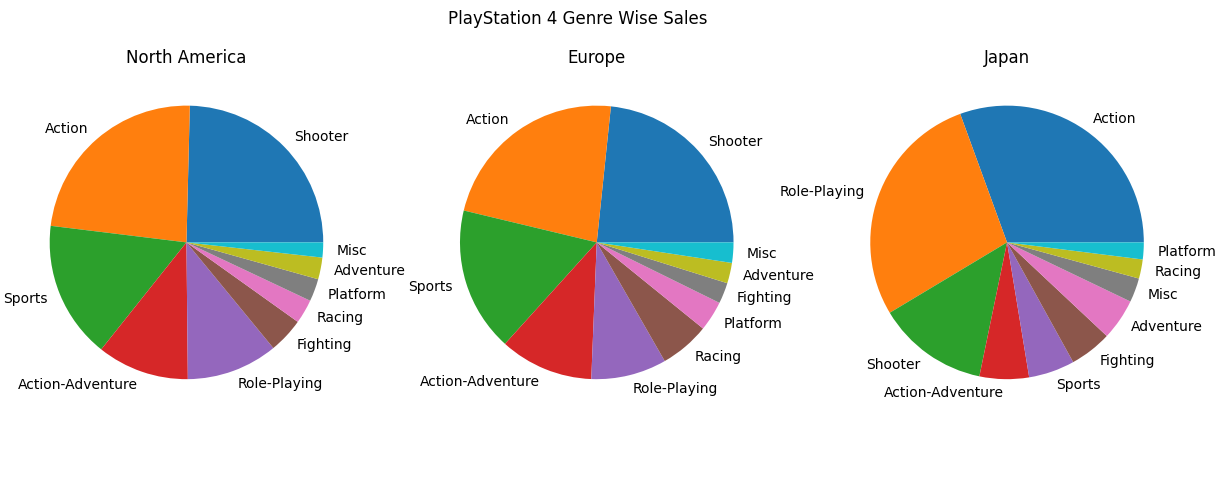
\includegraphics[width=0.5\textwidth]{regionplatformps4.png}
    \caption{PlayStation 4 Region Wise Top Selling Genres}
\end{figure}

\begin{figure}[h]
    \centering
    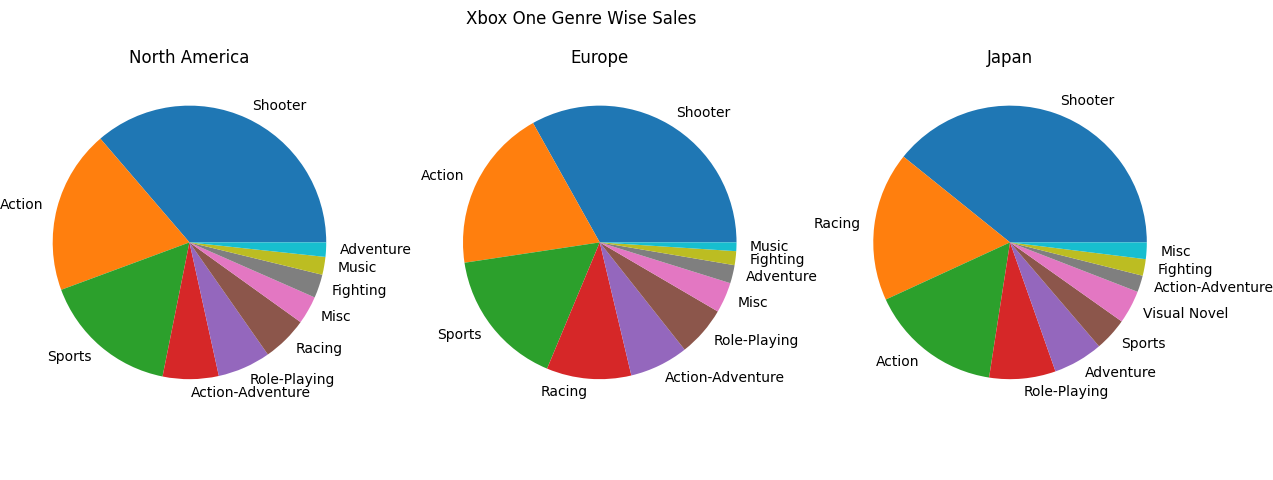
\includegraphics[width=0.5\textwidth]{regionplatformxb1.png}
    \caption{Xbox One Region Wise Top Selling Genres}
\end{figure}

\section{Problem Statement}
Video Game Industry is a billion-dollar business, and it has been since many years. Many companies have been dipping their toes into this business over many years and have accomplished so much. However, there are very few sales analytics available globally. Any industry participating in this side of business must first perform the feasibility, valuation etc. check for their product, Which is why a good analysis sales of over the past few years is very much required.\\
Another major player generating the revenue in the industry is the consoles. For that, Will it be appropriate making the game exclusive to certain consoles, and would it drag more people to buy the console and help build a good relationship with the respective console company?
\section{Proposed Solution}
For the approximation of the sales, We perform the analytics on the past data available one the video games sales. This would provide an approximated forecast for the companies along with how well it will do in certain regions and genres. Then for the second part, We begin our analysis on the console sales and analyse the impact of exclusive games on the sales of the consoles. \\
We started the forecasting of the sales by first cleaning the dataset and decomposing the time series data. We then plotted the decomposition and analysed the trend, seasonality and residuals. As we can see from the figure below, dataset contains no seasonality.\\
\begin{figure}[h]
    \centering
    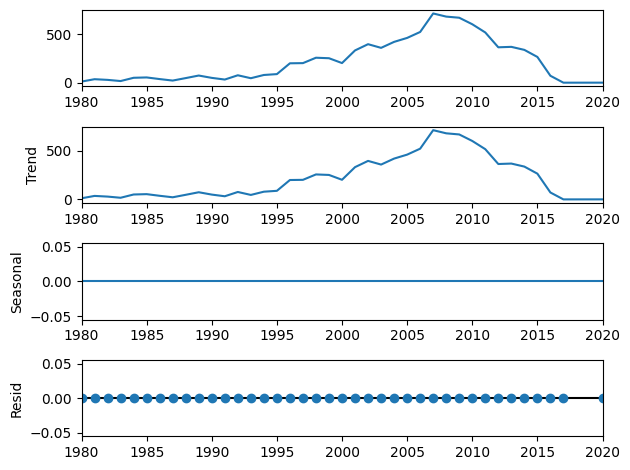
\includegraphics[width=0.5\textwidth]{decompose.png}
    \caption{Seasonality Decomposition of the dataset}
\end{figure}
Then we fitted the ARIMA model. The model was trained on 80 percent of the data, rest was used for the validation. The forecast using the model is given in the figure below.\\
\begin{figure}[h]
    \centering
    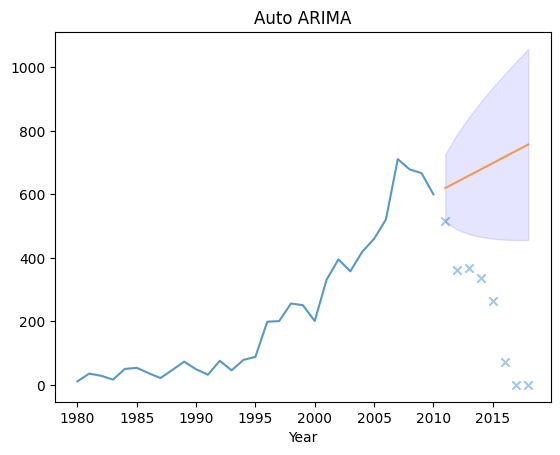
\includegraphics[width=0.5\textwidth]{before merge arima.png}
    \caption{ARIMA forecasts on the dataset}
\end{figure}
Here, the forecast seems very different from how it should be. For obvious reasons the accuracy is also very poor (RMSE 501.80). And the reason for this is quite obvious, there is a sudden steep decline in the sales. The reason for this is the dataset containing the data till 2016 and the consoles column did not include the newly launched consoles. So essentially, the downfall was the deprecation of the older consoles which is very normal. We performed a quick downfall of sales forecast as well using the MA (Moving Average) model, which is given in the figure below.\\
\begin{figure}[h]
    \centering
    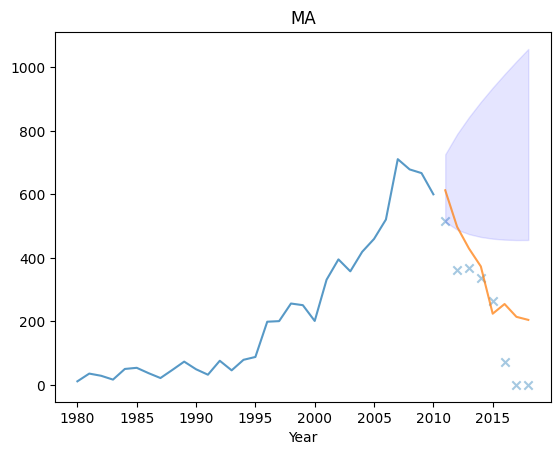
\includegraphics[width=0.5\textwidth]{downfall pred.png}
    \caption{Prediction of the downfall of older generation consoles}
\end{figure}
Now the question again arises, How will we be able to best approximate the sales. We answered this question by analysing a newer dataset that is merged with the older dataset. The newer datasets are the sales of the PlayStation 4 games and another one being sales of Xbox One games. Reason why we chose these datasets was very simple, both consoles were the highest grossing consoles and proportionally they, together drive the highest sales in the industry. The data made sense since as we can see in the figure below, sales are increasing year wise.\\
\begin{figure}[h]
    \centering
    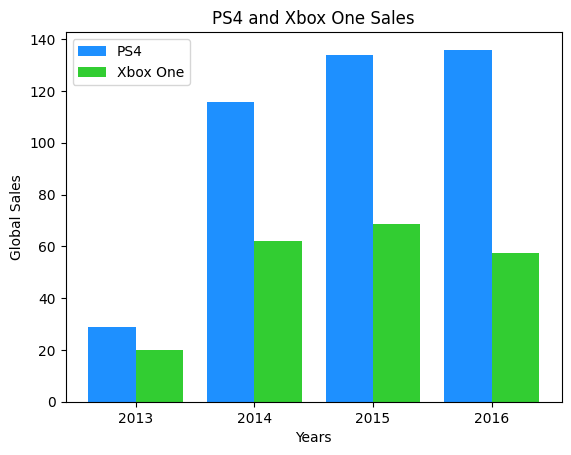
\includegraphics[width=0.5\textwidth]{merged.png}
    \caption{Year wise sales of video games in the newer datasets}
\end{figure}

This resulted into a much better approximation of the sales and provided very good accuracy. The model we used for this forecast was again ARIMA, and the forecasts are shown in below figure.\\
\begin{figure}[h]
    \centering
    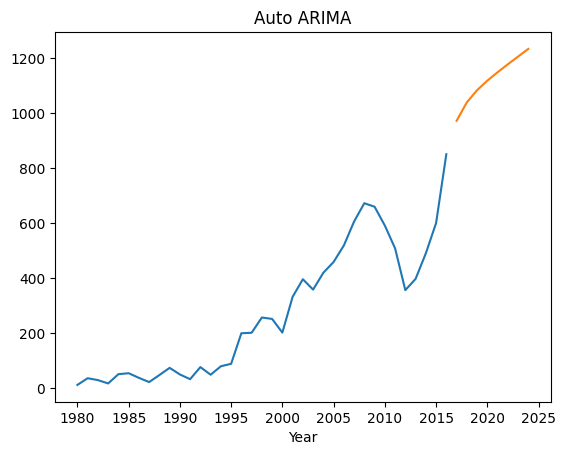
\includegraphics[width=0.5\textwidth]{merged pred.png}
    \caption{Sales forecast using ARIMA model with the merged dataset}
\end{figure}
For obvious reasons there is a small period of decline in the dataset, but that is due to the dataset having a gap in the time. But the model so far, was trained on this new merged dataset and gave us a very realistic climbs of sales and hence we can definitely conclude that the forecasts can be made according to this model for any particular company.\\
Now, we begin proposing the solution for the second phase of the problem. Let us get thorough with the problem first. The proportion of sales, the exclusive games are having is one way to solve this problem. But of course, we need to get a little closer to the solution here. Now one limitation for answering this problem is we cannot analyse the sentiment and thought-process of the customers when it comes to analysing the data, Essentially what I mean by this is we cannot have a column containing the "reason" for which, the user has purchased the respective console. For such reasons, we would rather divide this problem into two parts. One being the proportion of the sales of exclusive games on the total sales, and another being proportion of the revenue generated by those exclusive games on the console sales.\\
We began the analysis by performing data pre-processing in the newer videogames sales dataset. This was performed on the newer datasets (PS4 and Xbox One Videogames sales) since it is more appropriate to analyse the exclusivity on a newer dataset. After the pre-processing, we grouped the sales of games based on the years.\\
Now for the PlayStation 4, we chose Uncharted, Spider, God of, Bloodborne, Knack, Infamous, inFAMOUS, DriveClub, The Last of Us, MLB, Until Dawn, Gravity Rush, Tearaway, The Order, Ratchet and Horizon as the exclusive games and aggregated their sales. Similarly for Xbox One, we chose Halo, Sea of Thieves, Forza, Sunset Overdrive, Dead Rising 3 and Gears of War as exclusive titles and again aggregated their sales. After the computing the total sales, we performed the same grouping and aggregation on respective consoles but for this time, we excluded the exclusive games. This resulted into a visual representation of the proportion of the sales of exclusive games in the sales of all the games for their respective platform. The bar graph is given below.\\
\begin{figure}[h]
    \centering
    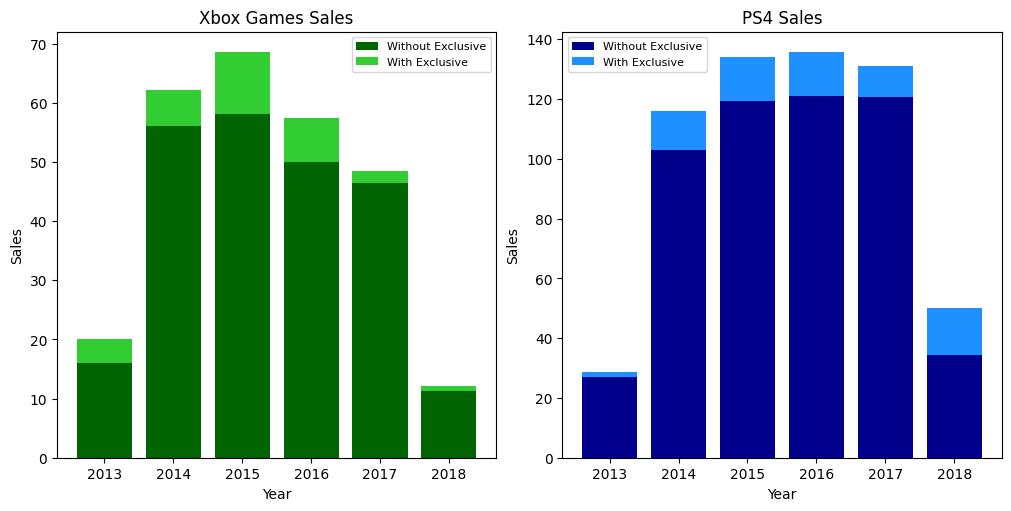
\includegraphics[width=0.5\textwidth]{excl1.png}
    \caption{Proportion of exclusive games sales on total sales}
\end{figure}
Then as discussed above, we began second part of the solution for tackling the problem statement better. We pre-processed the console dataset. Which contained both new and old generation of consoles. We again picked the highest grossing platforms among them, PlayStation 4 and Xbox One. We calculated the total sales for individual platform and plotted that on a bar graph. Then we again calculated the sales generated by only the exclusive games in millions, and stacked them on top of their respective console sales. The plot is given in the figure below.\\
\begin{figure}[h]
    \centering
    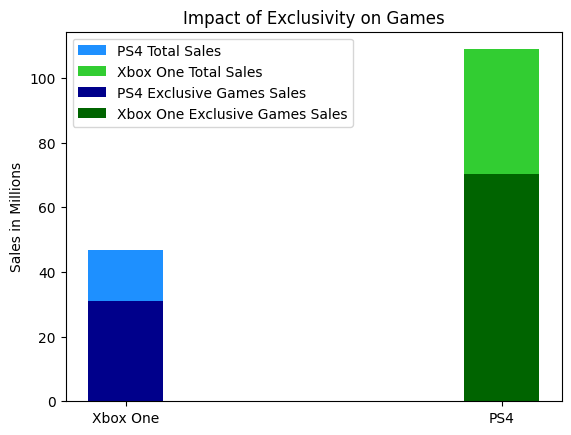
\includegraphics[width=0.5\textwidth]{excl2.png}
    \caption{Impact of sales of exclusive sales on respective console sales}
\end{figure}
Now, after performing these two analysis, we can see from the image as the time goes, the impact of exclusivity was increasing in both the platforms. In year 2015, it was recorded the highest. Then since the total sales were going down it started to go down but the important point to note here is, the trend of exclusive games was on peak in year 2015. The reason being most demanded and most popular platform specific video games were released in that year. Which indeed gave a significant impact on the total sales. As we can see above, we only took few games and compared to the entire population of the games, these few games themselves drew such big chunk of the sales. And for the consoles, we can see from the second plot, we can easily conclude that the exclusive games does have a significant impact on the console sales. Around 30 percentage of the revenue compared to the console revenue is generated by the exclusive games itself. Now mind the difference in the price of a game and the console too! So, this was the closest we can get for proposing a solution to the second part of the problem statement.

\section{Acknowledgment}
We would like to convey our gratitude to Dr. Nage Gowda for his support and assistance in the completion of this project. We would also like to thank the Computer Science and Engineering Department of PES University for encouraging us with this wonderful opportunity to work on a real world data analysis project. We are also thankful to the Teaching Assistants for their involvement and contribution in this course and help us interactively learn new concepts.

\begin{thebibliography}{00}
    \bibitem{b1} Witkowski, Wallace (December 26, 2020). "Videogames are a bigger industry than movies and North American sports combined, thanks to the pandemic". Market Watch. Retrieved December 27, 2020.
    \bibitem{b2} VGChartz, \textbf{``Video Games Sales''} \textit{\url{vgchartz.com}}
    \bibitem{b3} GregorUT, \textbf{``vgsales''} \textit{\url{https://www.kaggle.com/datasets/gregorut/videogamesales}}
    \bibitem{b4} Jaime Paz Lopez, \textbf{``Video Games Sales Dataset''} \textit{\url{https://www.kaggle.com/datasets/jaimepazlopes/game-console-manufactor-and-sales}}
    \bibitem{b5} Wikipedia, \textbf{``List of best selling game consoles''} \textit{\url{https://en.wikipedia.org/wiki/List_of_best-selling_game_consoles}}
    \bibitem{b6} Feray Adigüzel, \textbf{``The Effect of YouTube Reviews on Video Game Sales''} \textit{Article  in  Journal of Business Research - Turk · September 2021}
    \bibitem{b7} Jeffry Babb, Neil Terry, Kareem Dana, \textbf{``The Impact Of Platform On Global Video Game Sales''} \textit{Volume 12, Number 10, International Business \& Economics Research Journal – October 2013}
    \bibitem{b7} Yannan Niu, \textbf{``SWOT Analysis on Sony's PlayStation Under COVID-19''} \textit{ICMETSS 2021}

\end{thebibliography}
\end{document}
